\subsection{Coverage-Maximizing Reach Set Aproximation}\label{s:chaoticReachSet}

\paragraph{Motivation:} Design of calculation method for \emph{Reach Set Approximation} guarantying high \emph{Maneuverability}.

\paragraph{Background:}There is \emph{Coverage Ratio} property of \emph{Reach Set} (def. \ref{def:coverageRatio}). It has been shown that creating \emph{Reach Set} via \emph{greedy approach} is not feasible due to the \emph{Scaling Factor}.  \emph{Contracted Expansion} (sec. \ref{s:constrainedTrajectoryExpansion}) is enabling to apply selection criteria while building \emph{Reach Set} in given \emph{Cell}. 

The \emph{Cell} $cell_{i,j,k}$ has a center and walls from UAS viewpoint: a front wall, back wall (for $layer > 1$), a top wall, left wall, right wall, bottom wall. It is expected that trajectory leading close to one cell walls will continue to a different cell, increasing the chance to obtain more \emph{Unique Footprints}. 

\paragraph{Expansion Constraint Function Implementation} (alg. \ref{alg:ExpansionConstraintFunctionForChaoticReachSet}) is based on the simple principle: \emph{Select candidate Nodes which are  closest to outer walls of Cell, with a unique footprint}.

\paragraph{Tuning Parameters:} \emph{Proximity to Cell outer wall} gives good chances to break into other rows or columns in the \emph{Avoidance Grid}. \emph{Unique footprint} guarantees future \emph{Unique Footprint} after appending Trajectory by \emph{Movement application}. 
\begin{enumerate}
    \item \emph{Considered Footprint Length} - how much last cells in footprint should be considered in unique path track, minimal value 1, default value 3, maximal value $\infty$. If there is a need to generate non-redundant trajectories use $\infty$, it will consider full footprint.
    
    \item \emph{Spread Limit} - the upper limit of candidates which are going to be select for further expansion, minimal value 1, default value \emph{Count of unique Moves in Movement set}, maximal value $\infty$. If more than default values are selected, the algorithm will generate \emph{redundant trajectories}. If less is selected, then some trajectories are omitted, and \emph{Coverage Rate} decreases sharply. 
\end{enumerate}

\paragraph{Step: Initialization} initialization of \emph{candidate} array (return value), \emph{leftovers} array (return Value). Node array \emph{passing} is populated with \emph{Nodes} which represents \emph{end node of Trajectory}, and the tip of the  \emph{trajectory is constrained in the \emph{cell}$_{i,j,k}$}.

\paragraph{Step: Evaluate best trajectories with unique Footprints} following steps are executed:
\begin{enumerate}
    \item \emph{Best Performance Map} is created with a \emph{footprint} as a key set element to ensure footprint uniqueness.
    
    \item \emph{Wall distance} for the \emph{test node} is calculated as a closest trajectory portion distance to the \emph{top, bottom, left, right} wall of the $cell_{i,j,k}$
    
    \item The \emph{Footprint} for the \emph{test node} is created with the  maximal length given by \emph{Footprint Length} tuning parameter.
    
    \item \emph{Existence and Performance Test} is executed to ensure that the best performing node is selected. If there is no key entry in the \emph{Best Performance Map}, then a new entry for \emph{Test Node} is created. If there is a key entry, the performance of \emph{Old Node} and \emph{Test Node} is compared, and better is stored.
\end{enumerate}

\paragraph{Step: Select candidates} is executed on \emph{Best Performance Map} records using  \emph{Wall distance} as pivot parameter, ordering by closest proximity and limited by \emph{Search Limit} tuning parameter. The \emph{Leftovers} are difference set between \emph{Passing Nodes} and \emph{Candidate Nodes}. 


\begin{algorithm}[H]
    \SetKwInOut{Input}{Input}\SetKwInOut{Output}{Output}\SetKwInOut{TuningParameters}{Tuning Parameters}
    \Input{Node[] stack, Cell cell$_{i,j,k}$}
    \TuningParameters{int$^+$ footprintLength, int$^+$ spreadLimit}
    \Output{Node[] candidates, Node[] leftovers}
    
    \BlankLine
    \# Initialize structures\;
    Node[] candidates = [], Node[] leftovers=[]\;
    Node[] passing = cell$_{i,j,k}$.getFinishingTrajectories(stack)\;
    
    \BlankLine
    \# Select best performing trajectories with unique footprint\;
    Map$<$Footprint,Node$>$  bestPerformanceMap\;
    \For{Node test $\in$ passing}{
        wallDistance= test.minimalDistanceToWall(cell$_{i,j,k}$)]\;
        footPrint = test.getFootprint(lastCells = footprintLength)\;
        \eIf{bestPerformanceMap.contains(footPrint)}{
            old = bestPerformanceMap.getByKey(footprint)\;
            oldPerformance= old.minimalDistanceToWall(cell$_{i,j,k}$)\;
            \If{oldPerformance $>$ wallDistance}{
                bestPerformanceMap.setByKey(footprint,test)\;         
            }
        }{
            bestPerformanceMap.setByKey(footprint,test)\;
        }
    }
    
    \BlankLine
    \# Select best performing nodes up to \emph{spreadLimit} count\;
    candidates = bestPerformanceMap.select(count = spreadLimit).orderBy('wallDistance','Ascending')\;
    leftovers = passing - candidates\;
    \Return{[candidates,leftovers]}
    
    
    \caption{Expansion Constraint function for \emph{Coverage-Maximizing Reach Set Approximation}}
    \label{alg:ExpansionConstraintFunctionForChaoticReachSet}
\end{algorithm}


\paragraph{Example:} for \emph{Avoidance Grid} with \emph{Distance 10 m}, \emph{Layer count 10}, \emph{Horizontal range $[-45^\circ,+45^\circ]$}, \emph{Horizontal Cell Count 7}, \emph{Vertical range $[-30^\circ,+30^\circ]$}, and \emph{Vertical Cell Count 5}. Is given in (fig. \ref{fig:chaoticReachSetApproximation}). The UAS is at \emph{Back-side} of \emph{Figure} (initial state is at all \emph{Trajectory Origins}). The \emph{black dashed line} marks \emph{Avoidance Grid} space boundary. Each trajectory has its own color and ends at \emph{Front-side} of \emph{Avoidance Grid Boundary}.

\begin{figure}[H]
    \centering
    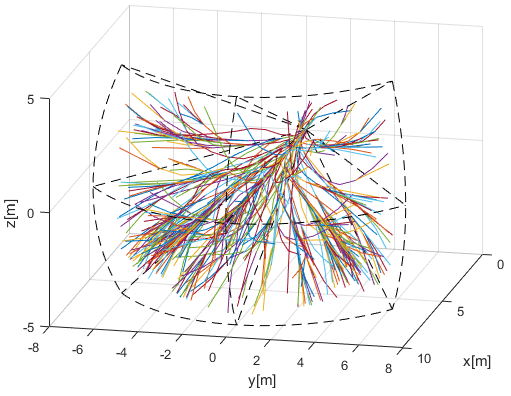
\includegraphics[width=0.7\linewidth]{\FIGDIR/RS002ChaoticReachSetEstimationMethod} 
    \caption{\emph{Coverage-Maximizing \emph{reach set} approximation}.}
    \label{fig:chaoticReachSetApproximation}
\end{figure}


\paragraph{Pros and Cons:} It can be seen from example (fig. \ref{fig:chaoticReachSetApproximation}) that \emph{Coverage-Maximizing Reach Set Approximation Method} (alg. \ref{alg:ExpansionConstraintFunctionForChaoticReachSet}) generates much \emph{turning} and \emph{shaky} \emph{trajectories}. 

\emph{High Coverage Ratio} ($\sim 0.9$) is provided while keeping \emph{medium node count}. The calculation complexity scales linearly with grid size. The \emph{upper limit of trajectories} is given as follow:

\begin{multline}
    countTrajectories(ReachSet) \le layerCellCount \times spreadLimit\\ \times size(Movements)
\end{multline}

\noindent The \emph{upper limit of nodes} is given as follow:
    
\begin{multline}
    countNodes(ReachSet) \le layerCount \times  layerCellCount  \\
    \times size(Movements) \times spreadLimit  
\end{multline}

\noindent The \emph{absence} of \emph{Smooth Trajectories} disqualifies \emph{Coverage Maximizing -RSA} to be used for \emph{Navigation}. This type of reach set is feasible for \emph{Avoidance} because it contains a variety of maneuvers.


